\documentclass[10pt]{article}
\usepackage[margin=1in]{geometry} 
\usepackage{enumerate, xfrac, color, graphicx}
\usepackage{amsmath,amsthm,amssymb,amsfonts,mathabx}
\usepackage{booktabs}
\usepackage{caption}
\usepackage{algorithm}
\usepackage{algpseudocode}
\usepackage{pifont}
\usepackage{listings, courier}
\graphicspath{{/Users/mfzhao/Dropbox/}}
\newcommand{\N}{\mathbb{N}}
\newcommand{\Z}{\mathbb{Z}}
\lstset{breaklines=true, basicstyle=\small\ttfamily, language=R, backgroundcolor=\color{highlight}, stepnumber=5}

\definecolor{highlight}{RGB}{248,248,248}

\begin{document}
	\title{6.867 Problem Set 3}
	\maketitle
	
\subsubsection*{Neural Networks}

We might want to use a neural network rather than another algorithm, such as SVM or logistic regression, in order to be somewhat more agnostic about the parametric form of the data-generating process. In this case, we investigate the use of neural networks, first on some toy training data sets, and subsequently on a subset of the popular MNIST dataset.

Let us first briefly review the way that neural networks works. Neural networks are inspired by how brains process information. In the brain we have interconnected neurons that produce electrochemical impulses that feed into other neurons. In a neural network, we try to mimic this architecture by using interconnected ``perceptrons" or nodes. These nodes are organized into ``layers" which are connected to nodes in other layers, but not to nodes in the same layer. 

In a feed-forward neural network (the specific type of neural network architecture we are working with), the outputs of each layer are fully connected to the next layer. These layer to layer connections are represented by a weight matrix. Functionally, the weight matrix produces a weighted linear combination of the outputs of a layer to use as the input for the next layer. This weighted linear combination is then fed into some nonlinear ``activation function" on each node (typically a sigmoid function or tanh function) which produces the output of a node. Its important to note that the activation function needs to be nonlinear, otherwise we would end up with a standard linear model (a linear combination of linear functions is still a linear function). These outputs can then be fed into a new layer via the same procedure as above. We can arbitrarily choose how many of these interconnected layers we want to include in a neural network model. 

\begin{figure}[ht]
	\centering
	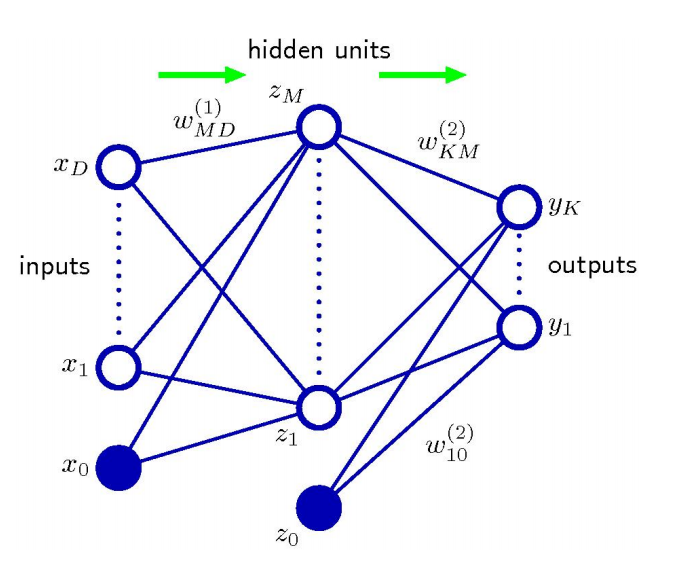
\includegraphics[height=3in]{neuralnetdiagram.png}
	\caption*{Figure 1: A schematic diagram of a neural network (taken from the homework assignment document)}
\end{figure}

Neural network models at the very least need two layers, an input layer and an output layer. These layers are constructed from  data, where the input layer is composed of features and the output layer is the label. In this sense, the simplest neural network  with a single node in the output layer is just a logistic regression. For networks with more than just the input layer and output layer, the intermediate layers are called ``hidden layers," since they're not directly observed (much like a hidden state in a Hidden Markov Model). A schematic sketch of a neural net with a single hidden layer can be found above. Alternatively, this neural network may be mathematically specified as follows:

\begin{equation}
a_{n}^{(1)} = \sum_d w_{dn}^{(1)}x_d
\end{equation}

\begin{equation}
z_{n}^{(1)} = f_1(a_n^{(1)})
\end{equation}

\begin{equation}
a_{k}^{(2)} = \sum_k w_{nk}^{(2)}z_n
\end{equation}

\begin{equation}
y_k = z_{k}^{(2)} = f_2(a_k^{(2)})
\end{equation}

\noindent Or in matrix notation:

\begin{equation}
a^{(1)} = X\cdot W^{(1)}	
\end{equation}

\begin{equation}
z^{(1)} = f_1(a^{(1)})
\end{equation}

\begin{equation}
a^{(2)} = z^{(1)}\cdot W^{(2)}	
\end{equation}

\begin{equation}
y = z^{(2)} = f_1(a^{(2)})
\end{equation}

For the purposes of this paper, we will try to solve simple multi-class prediction problems using a neural network with one hidden layer. In order to determine the weight matrices that give us the best predictive accuracy, we will specify a loss function and perform (batch or stochastic) gradient descent. We specify our objective function as the regularized negative log-likelihood function:

\begin{equation}
J(w) = l(w) +\lambda(||w^{(1)}||^2_F + ||w^{(2)}||^2_F
\end{equation}

\noindent where $l(w)$ is cross entropy loss:

\begin{equation}
l(w) = \sum_{i=1}^N \sum_{k=1}^{K} [-y_k^{(i)}\log(h_k(x^{(i)},w)) - (1-y_k^{(i)})\log(1-(h_k(x^{(i)},w))].
\end{equation}

To make our gradient descent faster, we want to use the analytical gradients of $w_1$ and $w_2$ for our gradient descent procedure. These gradients are calculated below.

\begin{equation}
\frac{\partial J(w)}{\partial w_{kj}^{(2)}} = \sum_{i=1}^N z_j \left(\sigma(a_k^{(2)}) -y_k^{(i)} \right) + 2 \lambda w_{kj}^{(2)}
\end{equation}

\noindent and 

\begin{equation}
\frac{\partial J(w)}{\partial w_{jd}^{(1)}} =  \sum_{i=1}^N x_i \sum_{k=1}^{K} \left(\sigma(a_k^{(2)}) -y_k^{(i)}\right) w_{kj}^{(2)} \left(\sigma(a_{jd}^{(1)})\right)\left(1-\sigma(a_{jd}^{(1)})\right) + 2 \lambda w_{jd}^{(1)}.
\end{equation}

\begin{table}
\captionof{table}{Neural Network Classification Error Rates With Various Parameters on Toy Datasets} 
\centering
\begin{tabular}{llllllll}
\toprule
Dataset & Method & $\lambda$ & $n_1$ = \bf{1} & $n_1$ =  \bf{3} & $n_1$ =  \bf{5} & $n_1$ =  \bf{7} & $n_1$ =  \bf{9} \\
\midrule
Toy Dataset 1 (Training) & full gradient descent & 0 &     0.007 & \bf{0}     & 0     & 0     & 0     \\
Toy Dataset 1 (Training) & full gradient descent & 1e-5 &   0.007 & 0     & 0     & 0     & 0     \\
Toy Dataset 1 (Training) & full gradient descent & 1e-3 &  0.093 & 0.003 & 0.003 & 0.003 & 0.003 \\
Toy Dataset 1 (Training) & full gradient descent & 1e-1 &  0.667 & 0.667 & 0.667 & 0.667 & 0.667 \\
\midrule
Toy Dataset 1 (Validation) & full gradient descent & 0 &      0.01  & \bf{0.003} & 0.003 & 0.003 & 0.003 \\
Toy Dataset 1 (Validation) & full gradient descent & 1e-5 &   0.01  & 0.003 & 0.003 & 0.003 & 0.003 \\
Toy Dataset 1 (Validation) & full gradient descent & 1e-3 &  0.063 & 0.003 & 0.003 & 0.003 & 0.007 \\
Toy Dataset 1 (Validation) & full gradient descent & 1e-1 &   0.667 & 0.667 & 0.667 & 0.667 & 0.667 \\
\midrule
Toy Dataset 1 (Training) & SGD & 0 &       \bf{0.003} & 0.003 & 0.003 & 0.003 & 0.003 \\
Toy Dataset 1 (Training) & SGD & 1e-5 &   0.043 & 0     & 0.003 & 0.003 & 0     \\
Toy Dataset 1 (Training) & SGD & 1e-3 &   0.117 & 0     & 0.003 & 0.003 & 0.003 \\
Toy Dataset 1 (Training) & SGD & 1e-1 &   0.667 & 0.667 & 0.667 & 0.667 & 0.667 \\
\midrule
Toy Dataset 1 (Validation) & SGD & 0 &       \bf{0.003} & 0.003 & 0.01  & 0.007 & 0.003 \\
Toy Dataset 1 (Validation) & SGD & 1e-5 &   0.033 & 0.007 & 0.003 & 0.007 & 0.003 \\
Toy Dataset 1 (Validation) & SGD & 1e-3 &   0.097 & 0.013 & 0.013 & 0.013 & 0.013 \\
Toy Dataset 1 (Validation) & SGD & 1e-1 &  0.667 & 0.667 & 0.667 & 0.667 & 0.667 \\
\midrule
Toy Dataset 2 (Training) & full gradient descent & 0 &      0.36  & 0.063 & 0.047 & 0.05  & 0.027 \\
Toy Dataset 2 (Training) & full gradient descent & 1e-5 &   0.397 & 0.063 & 0.067 & 0.063 & 0.067 \\
Toy Dataset 2 (Training) & full gradient descent & 1e-3 &  0.413 & \bf{0.06}  & 0.06  & 0.06  & 0.06  \\
Toy Dataset 2 (Training) & full gradient descent & 1e-1 &  0.667 & 0.667 & 0.667 & 0.667 & 0.667 \\
\midrule
Toy Dataset 2 (Validation) & full gradient descent & 0 &      0.343 & 0.07  & 0.093 & 0.1   & 0.107 \\
Toy Dataset 2 (Validation) & full gradient descent & 1e-5 &   0.39  & 0.073 & 0.07  & 0.073 & 0.073 \\
Toy Dataset 2 (Validation) & full gradient descent & 1e-3 &  0.38  & \bf{0.067} & 0.067 & 0.067 & 0.067 \\
Toy Dataset 2 (Validation) & full gradient descent & 1e-1 &  0.667 & 0.667 & 0.667 & 0.667 & 0.667 \\
\midrule
Toy Dataset 2 (Training) & SGD & 0 &       0.363 & 0.073 & 0.053 & 0.05  & 0.06  \\
Toy Dataset 2 (Training) & SGD & 1e-5 &   0.363 & 0.07  & \bf{0.067} & 0.057 & 0.067 \\
Toy Dataset 2 (Training) & SGD & 1e-3 &   0.363 & 0.07  & 0.07  & 0.07  & 0.07  \\
Toy Dataset 2 (Training) & SGD & 1e-1 &   0.667 & 0.667 & 0.667 & 0.667 & 0.667 \\
\midrule
Toy Dataset 2 (Validation) & SGD & 0 &       0.373 & 0.083 & 0.11  & 0.103 & 0.113 \\
Toy Dataset 2 (Validation) & SGD & 1e-5 &   0.373 & 0.087 & \bf{0.077} & 0.08  & 0.09  \\
Toy Dataset 2 (Validation) & SGD & 1e-3 &   0.377 & 0.097 & 0.097 & 0.093 & 0.093 \\
Toy Dataset 2 (Validation) & SGD & 1e-1 &   0.667 & 0.667 & 0.667 & 0.667 & 0.667 \\
\bottomrule
\end{tabular}
\end{table}

Let's now see how a neural network performs on two different toy data sets. We vary both the number of hidden nodes and the regularization parameter in our objective function, and use both full gradient descent and mini-batch stochastic gradient descent (with a batch size of 10). In particular, we use mini-batch SGD as opposed to full SGD (where batch size is 1) since mini-batch  has better convergence properties. The two algorithms perform comparably - in the case of toy data set number 2, we find that the full gradient descent algorithm does a slightly better job at finding the optimal values of our parameter than stochastic gradient descent (classification error of 6.7\% as opposed to 9\%). While full gradient descent does perform better, its important to note the SGD was significantly faster. This should be expected since full-batch uses the entire dataset to perform an update while SGD only uses a fraction, meaning that when we use SGD as opposed to full gradient descent we lose some of the nice convergence properties to gain faster updates. 

It's important to note that our changes in parameters have a much larger effect on the performance for toy dataset 2 than for our features in toy dataset 1. This is likely due to the fact that the second toy dataset is not linearly separable, as seen in the plots below. While a researcher can essentially achieve 100\% classification accuracy by drawing vertical lines to classify toy dataset \#1, there is overlap in the locations of our classes in toy dataset \#2. Consequently, the regularization constants have more influence on performance.

\begin{figure}[ht]
	\centering
	\begin{minipage}[b]{.48\linewidth}
		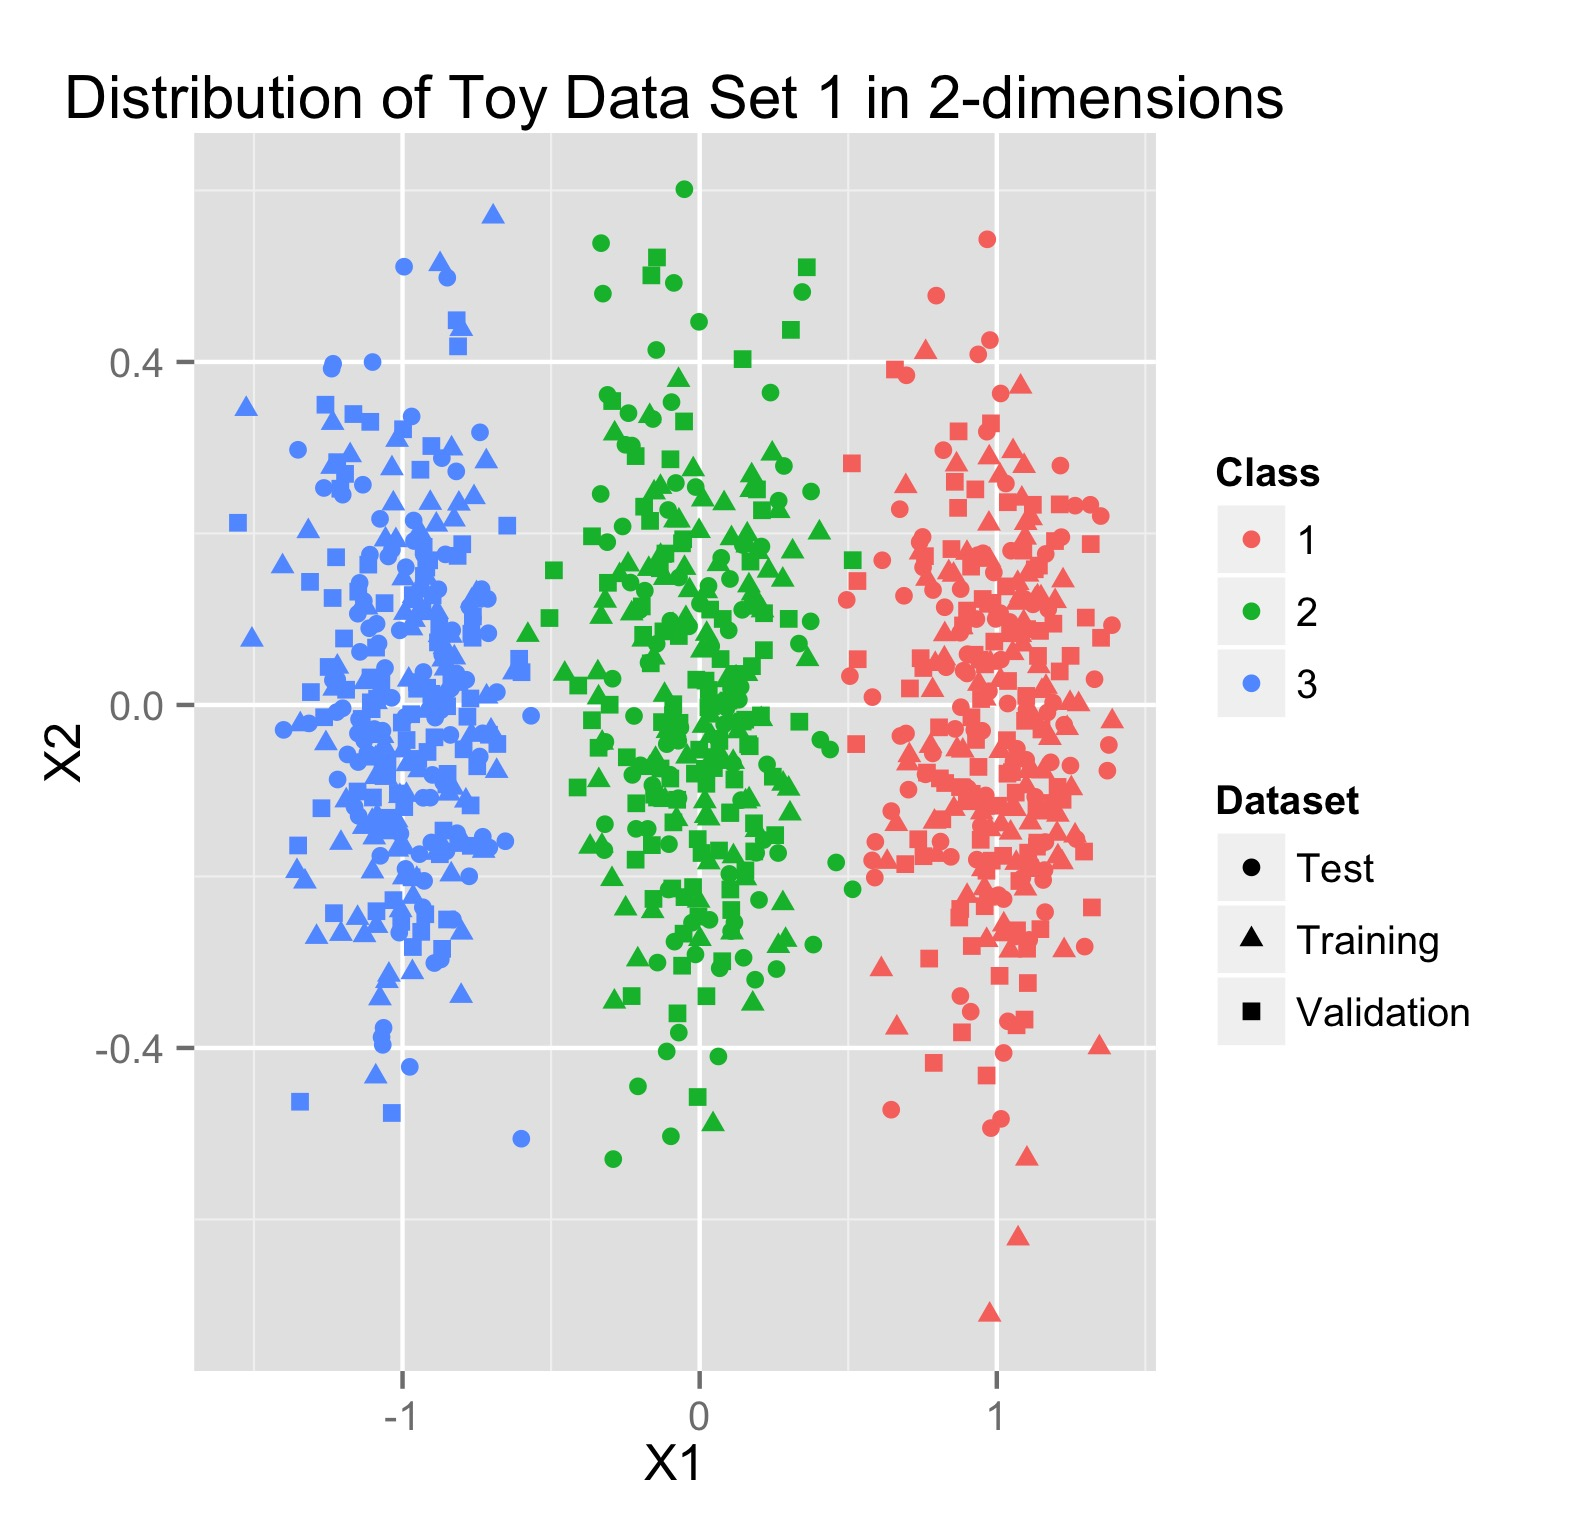
\includegraphics[width=1\linewidth, height=2.7in]{t1dist.jpg}
		\caption*{Toy Dataset \#1}
	\end{minipage}
	\begin{minipage}[b]{.48\linewidth}
		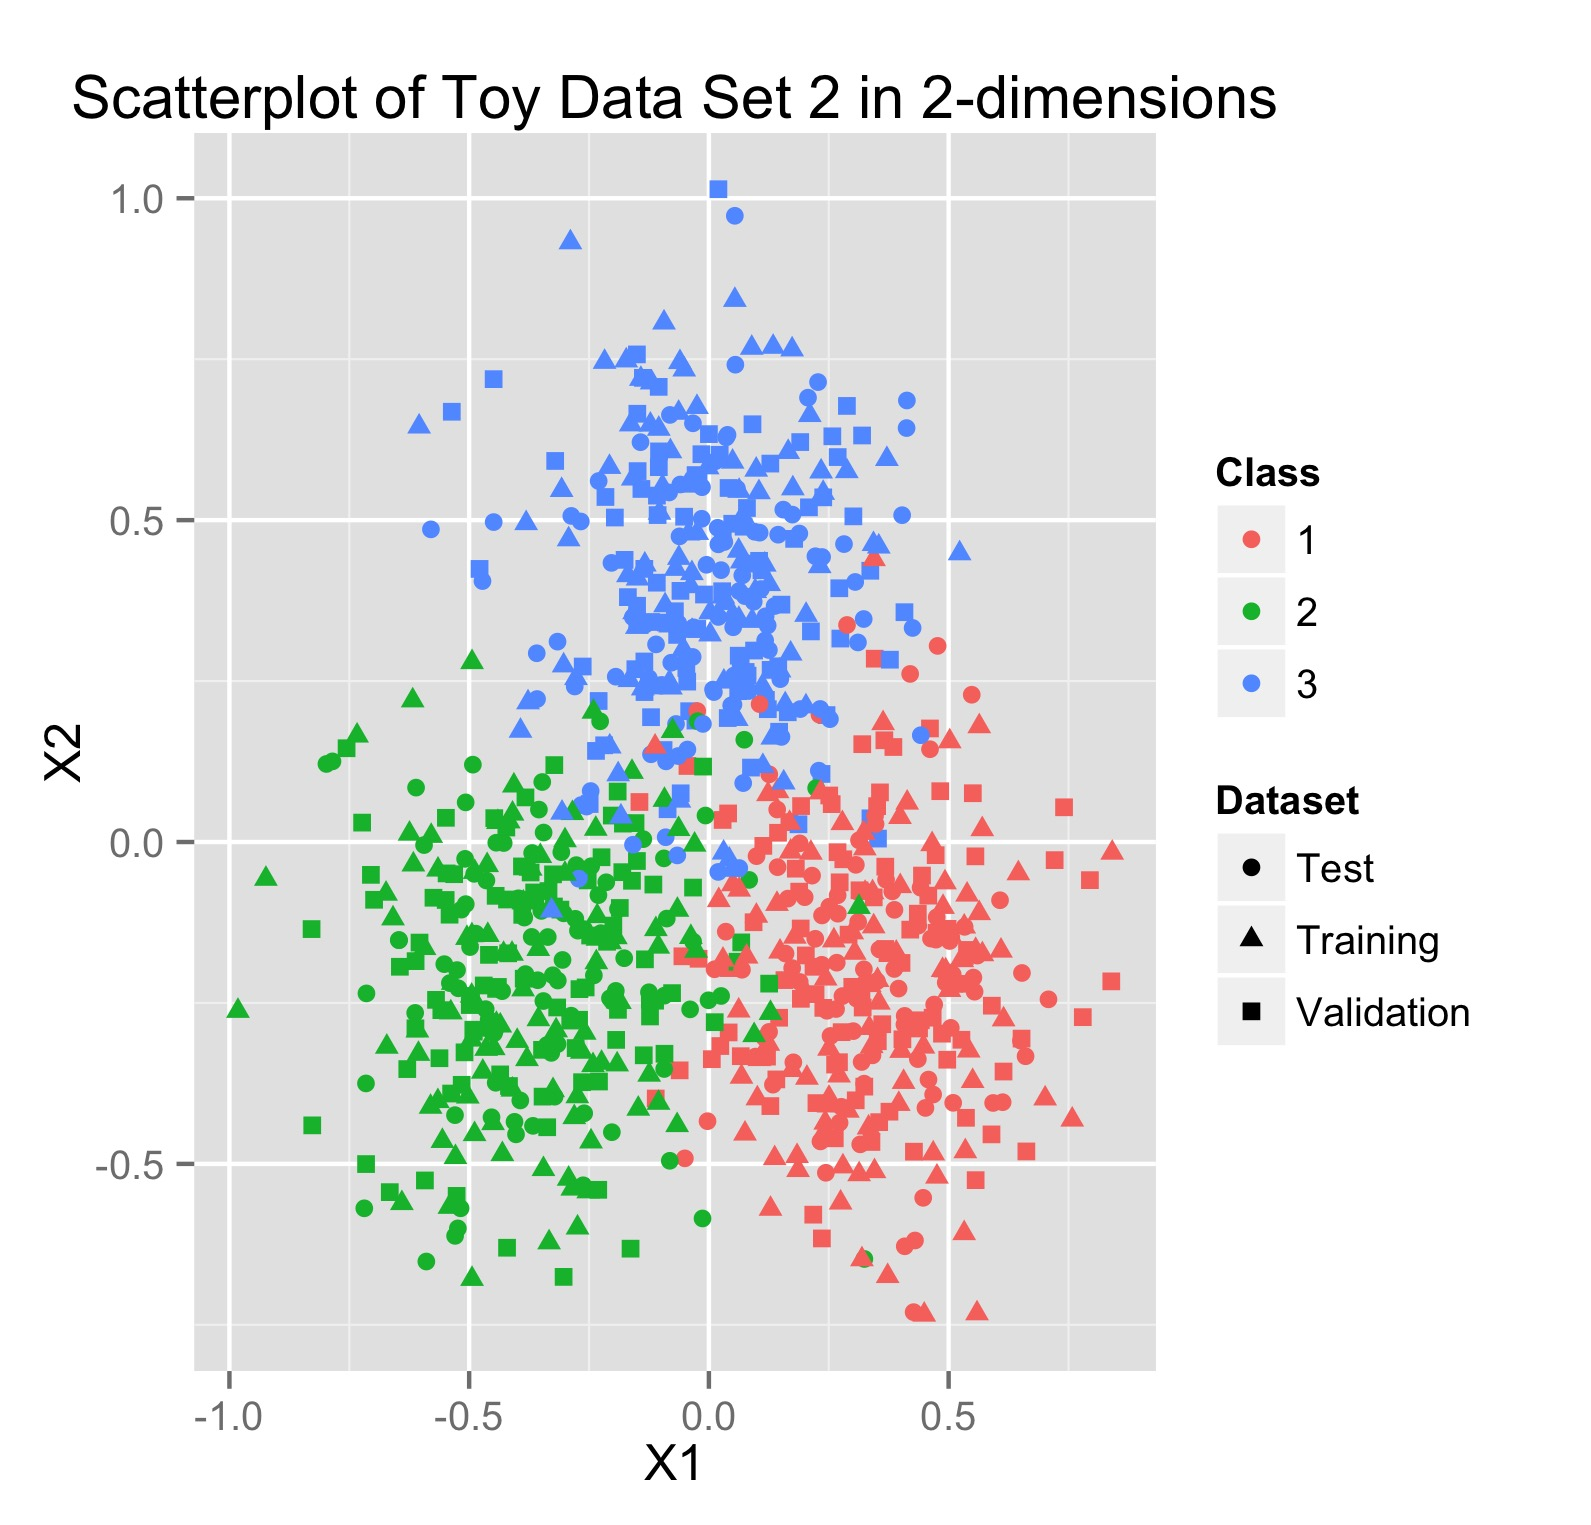
\includegraphics[width=1\linewidth, height=2.7in]{t2dist.jpg}
		\caption*{Toy Dataset \#2}
	\end{minipage}
	\caption{Scatterplots of different classes in $X1$, $X2$ for toy datasets}
\end{figure}

We are now interested in testing out neural network code on a real dataset. In our case, we're using a subset of the very popular MNIST data collected by Yann Lecunn. This dataset is comprised of 28 by 28 pixel images of handwritten digits with corresponding labels that represent what numbers these images actually represent. For our features, each 28x28 image is flattened into a feature vector of 784 where each of these features represent the darkness of a pixel (0 means that its a white pixel, 1 means its a black pixel, everything in between are shades of grey). Our dataset only consists of 6 distinct digits. 

When training on the MNIST data, we capped the number of iterations of our gradient descent (for both full batch and SGD) so that to convergence wouldn't take forever. Furthermore, in practice, this may serves as a way of preventing overfitting as long as we are still getting reasonably close. We again train both full-batch and stochastic gradient descent (batch size = 25) neural networks on the MNIST data, with a variety of different learning rates, regularization parameters and numbers of hidden nodes. The classification errors on both training and validation sets are found in Table 2, with best results in bold. 

\begin{table}
\captionof{table}{Neural Net Classification Error Rates on MNIST dataset for different choices of parameters} 
\centering
\begin{tabular}{llllllllll}
\toprule
Dataset & $lr$ & method & $\lambda$ & $n_1$ = 50 & $n_1$ = 100 & $n_1 = 150$ \\
\midrule
Training & .1 & full gradient descent &  0 & 0     & 0     & \bf{0}     \\
Training & .1 & full gradient descent & 1e-3 & 0.007 & 0.005 & 0.006 \\
Training & .1 & full gradient descent & 1e-2 & 0.069 & 0.069 & 0.074 \\
Training & .1 & full gradient descent & 1e-1 & 0.812 & 0.812 & 0.812 \\
\midrule
Validation & .1 & full gradient descent &  0 & 0.068 & 0.078 & \bf{0.062} \\
Validation & .1 & full gradient descent & 1e-3 &  0.064 & 0.07  & 0.062 \\
Validation & .1 & full gradient descent & 1e-2 & 0.072 & 0.078 & 0.078 \\
Validation & .1 & full gradient descent & 1e-1 & 0.822 & 0.822 & 0.822 \\
\midrule
Training & .1 & SGD &  0 & 0.112 & 0.109 & \bf{0.106} \\
Training & .1 & SGD & 1e-3 & 0.109 & 0.119 & 0.114 \\
Training & .1 & SGD & 1e-2 & 0.13  & 0.132 & 0.131 \\
Training & .1 & SGD & 1e-1 & 0.683 & 0.703 & 0.78  \\
\midrule
Validation & .1 & SGD &  0 & 0.09  & 0.1   & \bf{0.086} \\
Validation & .1 & SGD & 1e-3 & 0.092 & 0.09  & 0.098 \\
Validation & .1 & SGD & 1e-2 & 0.122 & 0.122 & 0.12  \\
Validation & .1 & SGD & 1e-1 & 0.68  & 0.698 & 0.762 \\
\midrule
Training & .01 & full gradient descent &  0 & 0.084 & 0.064 & 0.057 \\
Training & .01 & full gradient descent &  1e-3 & 0.076 & 0.067 & \bf{0.056} \\
Training & .01 & full gradient descent &  1e-2 & 0.094 & 0.087 & 0.081 \\
Training & .01 & full gradient descent & 1e-1 & 0.663 & 0.66  & 0.66  \\
\midrule
Validation & .01 & full gradient descent &  0 & 0.09  & 0.076 & 0.08  \\
Validation & .01 & full gradient descent & 1e-3 & 0.102 & 0.074 & \bf{0.07}  \\
Validation & .01 & full gradient descent & 1e-2 & 0.088 & 0.08  & 0.076 \\
Validation & .01 & full gradient descent & 1e-1 & 0.674 & 0.672 & 0.672 \\
\midrule
Training &.01 & SGD &  0 & 0.14  & 0.122 & 0.115 \\
Training &.01 & SGD & 1e-3 & 0.153 & 0.132 & \bf{0.124} \\
Training &.01 & SGD & 1e-2 & 0.153 & 0.152 & 0.138 \\
Training &.01 & SGD & 1e-1 & 0.629 & 0.545 & 0.511 \\
\midrule
Validation & .01 & SGD &  0 & 0.14  & 0.116 & 0.118 \\
Validation & .01 & SGD & 1e-3 & 0.136 & 0.126 & \bf{0.108} \\
Validation & .01 & SGD & 1e-2 & 0.128 & 0.142 & 0.124 \\
Validation & .01 & SGD & 1e-1 & 0.622 & 0.548 & 0.504 \\
\bottomrule
\end{tabular}
\end{table}

As expected, we see that SGD performs slightly worse than full-batch gradient descent, since it does not overfit as much. Our data seems to show that increasing the number of hidden nodes strictly increasing performance - this is not surprising, although we imagine that as you continue to increase $n_1$, you begin to get diminishing returns for increasing computational complexity. Decreasing the step size (i.e., smaller learning rate) also seems to lead us to achieve slightly better learning rates, although this causes the algorithm to require many more iterations to converge. A chart of the neural network classification error on the MNIST validation set can be found in Figure 2.

Note, however that we see the performance difference to be much more substantial than what we saw in the toy data. This is mostly the result of the 5000 iteration cap we imposed on the gradient descent procedure. Since we often hit the cap in while training, full-batch was considerably closer to convergence compared to the SGD as the each full-batch update more reliably and steadily decreases the loss. Again, however each SGD update was considerably faster than a full-batch update. If we allowed the SGD to continue a little longer, the results from our SGD probably would've considerably closer to the full-batch case. 

\begin{figure}[ht]
\center
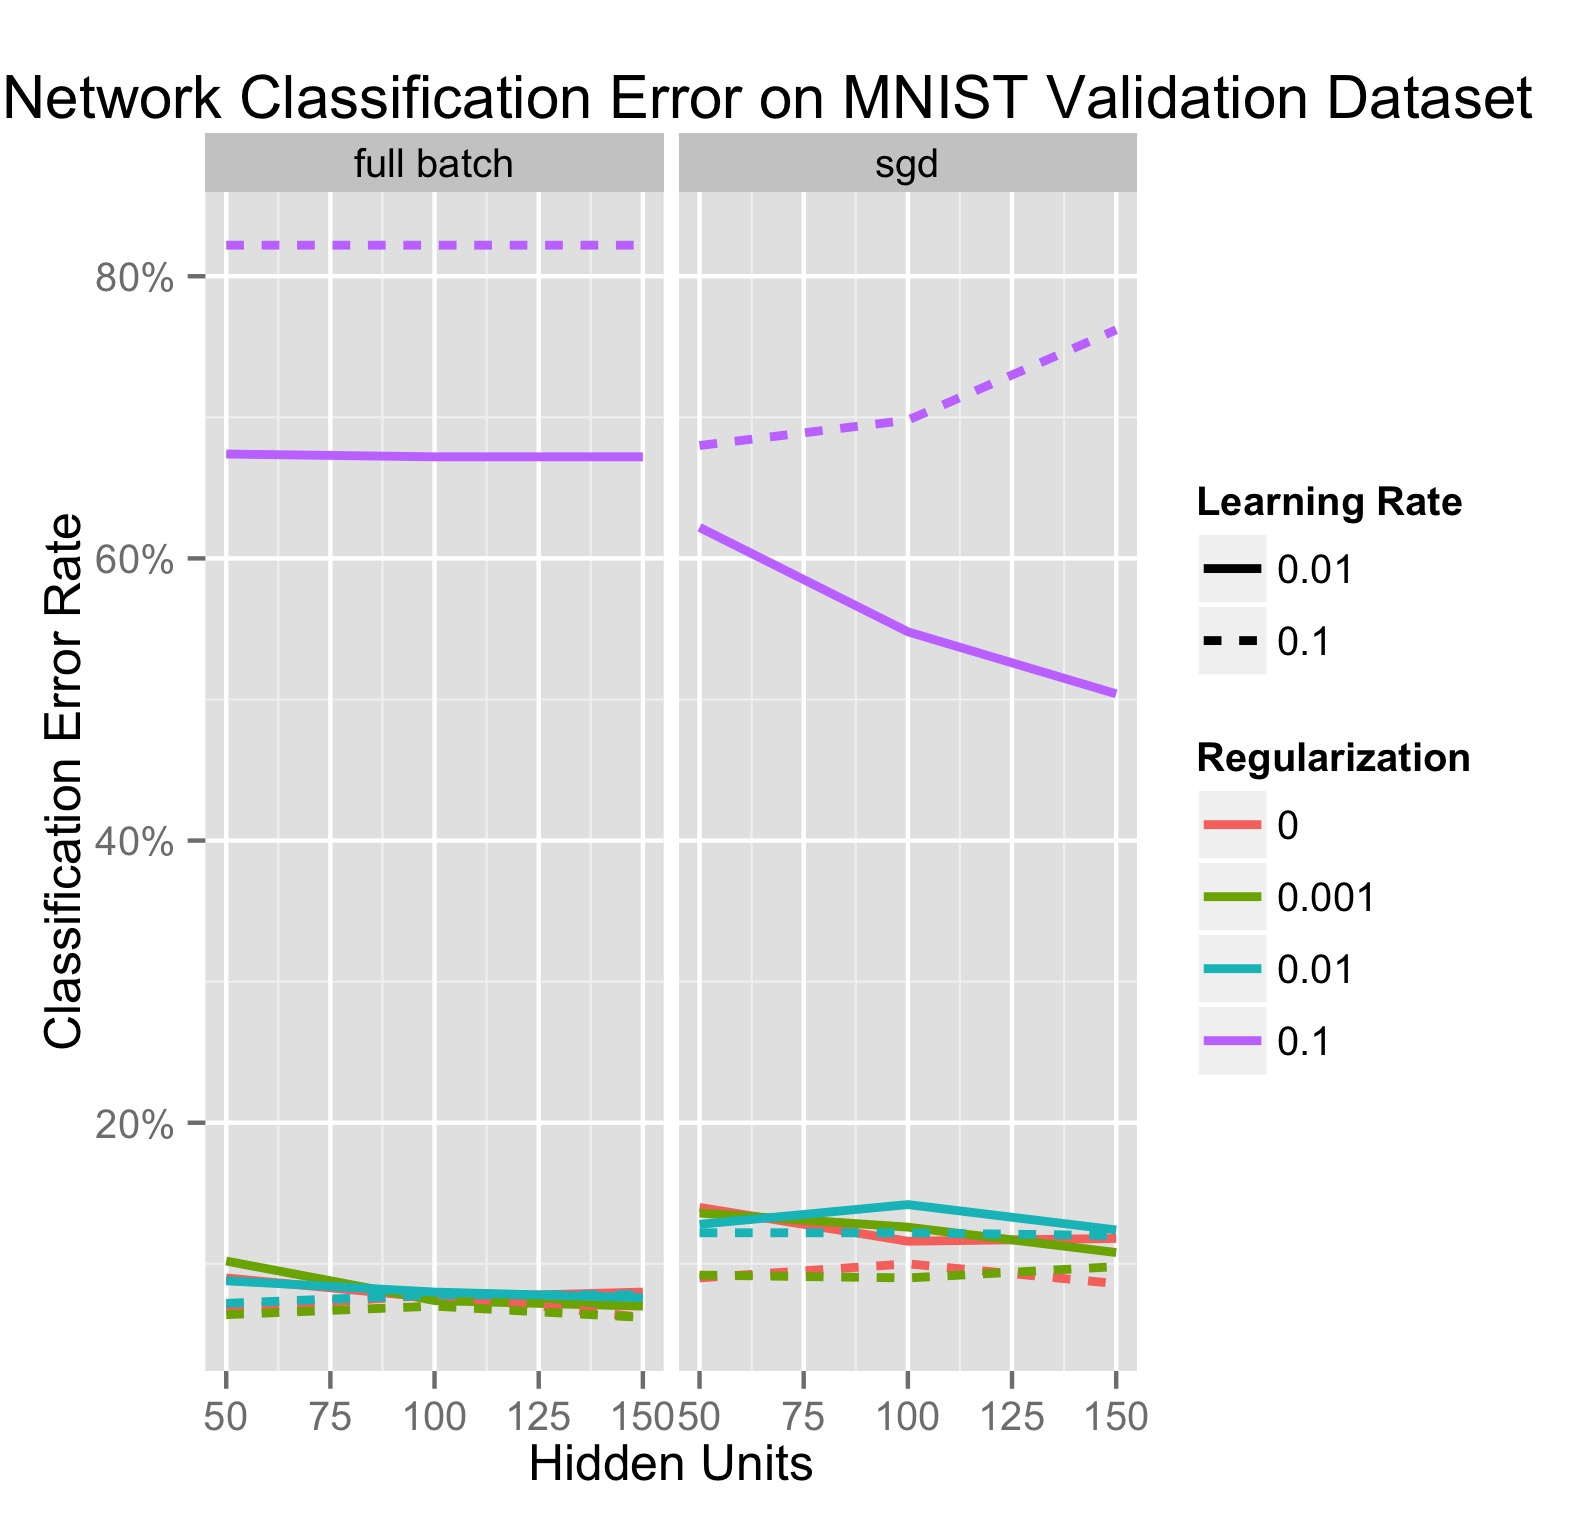
\includegraphics[height=4in, width=5in]{nnperf.jpg}
\caption*{Figure 2: Neural Network Classification Error on MNIST Validation Sets}
\end{figure}
	
\end{document}